% SemEval-2027 Task 3 system description paper -- official ACL template (acl.sty from
% github.com/acl-org/acl-style-files, commit d5adc82). Build: python scripts/build_report.py
% SemEval system papers are not anonymous: use [final]; [preprint] adds page numbers for a printed copy.
\documentclass[11pt]{article}
\usepackage[final]{acl}

\usepackage{times}
\usepackage{latexsym}
\usepackage[T1]{fontenc}
\usepackage[utf8]{inputenc}
\usepackage{microtype}
\usepackage{inconsolata}
\usepackage{graphicx}
\usepackage{booktabs}
\usepackage{array}
\usepackage{amsmath}
\usepackage{amssymb}
\usepackage{xcolor}
\usepackage{xspace}
\usepackage{tikz}
\usetikzlibrary{positioning,arrows.meta,fit,calc}

\input{author}  % generated from configs/author.json (team, name, affiliation, e-mail, optional notes)

\newcommand{\sys}{SiamGNN\xspace}
\newcommand{\xll}{XL-LEXEME\xspace}
\newcommand{\bcubed}{B$^3$-F1\xspace}
\newcommand{\std}[1]{{\scriptsize$\,\pm$#1}}
\definecolor{oursfill}{HTML}{E3EEFB}
\definecolor{oursdraw}{HTML}{2A78D6}

\title{\teamname{} at SemEval-2027 Task 3: Siamese Usage Graphs for\\Tracking Word Senses across Ten Time Periods}

\author{\authorname\authornote \\
  \programme, \facultyen \\
  \university, \city \\
  \texttt{\authoremail}}

\begin{document}
\maketitle

\begin{abstract}
We describe our system for SemEval-2027 Task~3, which asks systems to group the usages of a word into senses across ten time periods (Subtask~1) and to detect the usages of a given sense (Subtask~2). Starting from the standard pipeline of \xll embeddings and clustering, we propose \sys: a Siamese network whose usage representations are refined by message passing over a nearest-neighbour graph of all usages of a word. It is trained episodically on synthetic diachronic English to predict whether two usages share a sense, and its output is decoded with correlation clustering. For Subtask~2, the sense definition serves as a one-shot prototype that is refined with the closest usages. On held-out synthetic English words, a \sys ensemble gives the best sense-dynamics correlation (0.292 vs.\ 0.238 for the baseline), and message passing adds 0.08 (English) and 0.14 (Swedish) Spearman~$\rho$ over a Siamese-only head. On the Swedish development set, however, no \sys variant beats the \xll baseline with a transferred threshold (BCubed-F1 0.815, $\rho$ 0.523), which we trace to over-merged senses and an era gap in the embeddings. Prototype refinement raises Subtask~2 macro-F1 from 0.571 to 0.588.
\end{abstract}

% =====================================================================================
\section{Introduction}

Words gain, lose and redistribute senses over time. Computational work on lexical semantic change (LSC) has mostly compared two time periods and summarised change in one score per word \citep{schlechtweg2020semeval,tahmasebi2021survey}. SemEval-2027 Task~3 \citep{tahmasebi2027semeval} instead asks systems to model each sense across ten periods between 1880 and 2023, in Swedish, English, Italian, Spanish, Dutch and Russian. Subtask~1 is diachronic word sense induction: usages are grouped into senses (1a), and the resulting sense distributions must show when and for which words change happens (1b). Subtask~2 gives the definition of one target sense and asks which usages express it, mirroring how humanities researchers trace one concept through time.

The standard approach to sense-level LSC embeds every usage with \xll \citep{cassotti2023xllexeme}, a Siamese XLM-R bi-encoder trained on Word-in-Context (WiC) data, and clusters the embeddings \citep{periti2024systematic,periti2024towards}. Two weaknesses motivate our system: the number of senses hinges on a hand-tuned distance threshold, and every pair of usages is compared in isolation, ignoring the other usages of the word. \sys keeps the encoder frozen but learns the pairwise same-sense decision. Usages become nodes of a nearest-neighbour graph, two message-passing layers \citep{kipf2017semi,hamilton2017inductive} contextualise each usage with similar usages from all periods, and a Siamese head \citep{koch2015siamese} outputs a calibrated same-sense probability. The resulting graph is clustered with correlation clustering \citep{bansal2004correlation}, the objective used to derive the gold senses of diachronic word usage graphs \citep{schlechtweg2021dwug}. As the development data contain only ten Swedish words, we train episodically on synthetic diachronic English \citep{saponara2026generating}. For Subtask~2, the definition is a one-shot prototype that we refine transductively \citep{snell2017prototypical}.

On the development data we find that (i) message passing is what makes the learned similarity work, adding 0.08--0.14 Spearman~$\rho$ over a Siamese-only head; (ii) \sys gives the best sense dynamics on held-out synthetic English but does not beat the tuned \xll baseline on historical Swedish, a transfer gap that we trace to over-merged senses and to an era gap in the embeddings; (iii) the sense-dynamics score is fragile: shifting the clustering threshold by $\pm0.05$ for four of the ten Swedish words lowers $\rho$ from 0.523 to 0.303; and (iv) prototype refinement adds 1.7 macro-F1 points in Subtask~2. The evaluation phase takes place in January 2027, so this version of the paper reports development results only.\codefootnote

% =====================================================================================
\section{Background}

\paragraph{Task setup.}
For each target word $w$ the input is a set of usages, each a sentence with the character offsets of $w$, its year and a period label. In Subtask~1, a system assigns one or more integer sense labels to every usage, with no sense inventory given (\emph{The mouse ran across the floor}, 1885, and \emph{Click the mouse button}, 2015, should differ). Subtask~1a is scored with extended BCubed-F1 for overlapping clusters \citep{bagga1998entity,amigo2009comparison}, computed per word and macro-averaged. Subtask~1b is derived from the same labels: for every pair of consecutive periods, the scorer computes the Jensen--Shannon distance \citep[base 2;][]{lin1991divergence} between the two sense distributions, in which a usage with $m$ senses counts $1/m$ for each. The resulting $|W|\times(|T|-1)$ change scores of a language are ranked jointly and compared with the gold ranking by Spearman's~$\rho$; pairs in which either period has fewer than ten usages are skipped. Subtask~2 adds the definition of one target sense per word; systems output a binary label per usage, scored by macro-F1 over both classes per word and averaged over words. We take part in both subtasks.

\paragraph{Data.}
The development set is Swedish only: 10 words with 1,983 usages (98--291 per word) from ten periods, five from 1880--1915 newspapers with OCR noise and five from 2006--2023 news. Five words span both eras, \emph{skär} occurs only before 1915 and four words only after 2006. Each word has 3--12 gold senses (mean 5.7), 13\% of the usages carry more than one sense and 36\% express the Subtask~2 target sense. The test set has 130 words: 40 Swedish, 30 English and 15 each for Italian, Spanish, Dutch and Russian. As the only additional resource we use the synthetic English data of \citet{saponara2026generating}: a Llama-based generator fine-tuned on Oxford English Dictionary quotations writes usages of OED senses for ten 20-year periods from 1810, with realistic sense-frequency trajectories. We use 60 words for training (up to 15 usages per period, 8,775 usages, 4.0 senses per word) and 20 disjoint words for evaluation (2,850 usages, 3.65 senses).

\paragraph{Related work.}
Clustering contextual embeddings is the standard route to sense-level LSC \citep{giulianelli2020analysing,martinc2020capturing,periti2024lexical}. \xll outperforms other contextualised models on WiC, word sense induction and graded change \citep{periti2024systematic}, and \citet{periti2024towards} argue that LSC must move to many periods and diachronic sense induction. In the AXOLOTL'24 shared task on new-sense detection \citep{fedorova2024axolotl}, the best system combined gloss-based sense disambiguation with agglomerative clustering \citep{kokosinskii2024deepchange}, and graph-based clustering has been applied to semantic change across time and languages \citep{ma2024graphbased}. Gold LSC data are themselves usage graphs, annotated pairwise and clustered with correlation clustering \citep{schlechtweg2021dwug,schlechtweg2024sense}. Subtask~2 resembles target sense verification \citep{breit2021wictsv} and gloss-informed bi-encoders \citep{blevins2020moving}. We bring graph neural message passing and few-shot Siamese training into this pipeline, so that the usage graph itself is learned rather than built from fixed cosine similarities.

% =====================================================================================
\section{System Overview}

\begin{figure*}[t]
\centering
\resizebox{\textwidth}{!}{%
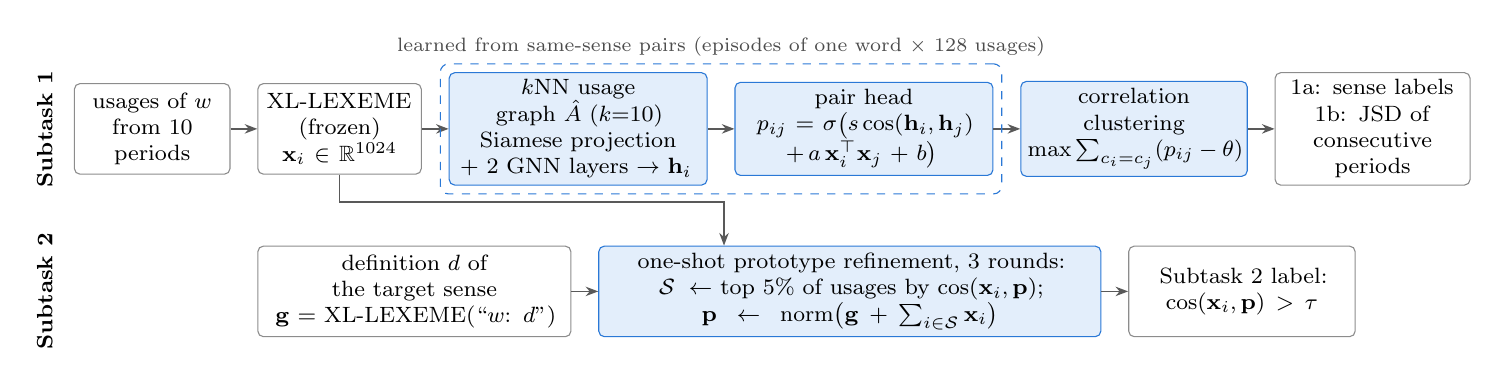
\begin{tikzpicture}[font=\footnotesize, node distance=3mm and 3.4mm,
  box/.style={draw=black!45, rounded corners=2pt, align=center, inner sep=2.5pt, minimum height=11.5mm},
  ours/.style={box, fill=oursfill, draw=oursdraw},
  arr/.style={-{Stealth[length=1.6mm]}, semithick, black!65},
  lane/.style={font=\footnotesize\bfseries, rotate=90, anchor=south}]
\node[box, text width=18mm] (u) {usages of $w$\\from 10 periods};
\node[box, text width=19mm, right=of u] (x) {\xll (frozen)\\$\mathbf{x}_i\in\mathbb{R}^{1024}$};
\node[ours, text width=31mm, right=of x] (mp) {$k$NN usage graph $\hat{A}$ ($k{=}10$)\\Siamese projection\\+ 2 GNN layers $\rightarrow\mathbf{h}_i$};
\node[ours, text width=31mm, right=of mp] (p) {pair head\\$p_{ij}=\sigma\big(s\cos(\mathbf{h}_i,\mathbf{h}_j)$\\$+\,a\,\mathbf{x}_i^{\top}\mathbf{x}_j+b\big)$};
\node[ours, text width=27mm, right=of p] (cc) {correlation clustering\\$\max\sum_{c_i=c_j}(p_{ij}-\theta)$};
\node[box, text width=23mm, right=of cc] (o1) {1a: sense labels\\1b: JSD of\\consecutive periods};
\foreach \a/\b in {u/x, x/mp, mp/p, p/cc, cc/o1} \draw[arr] (\a) -- (\b);
\node[draw=oursdraw, dashed, rounded corners=3pt, fit=(mp)(p), inner sep=3pt,
  label={[font=\scriptsize, text=black!70, yshift=-1pt]above:learned from same-sense pairs (episodes of one word $\times$ 128 usages)}] {};
\node[box, text width=38mm, below=9mm of x.south west, anchor=north west] (d) {definition $d$ of the target sense\\$\mathbf{g}=\text{\xll}(\text{``}w\text{: }d\text{''})$};
\node[ours, text width=62mm, right=of d] (pr) {one-shot prototype refinement, 3 rounds:\\$\mathcal{S}\leftarrow$ top 5\% of usages by $\cos(\mathbf{x}_i,\mathbf{p})$;\; $\mathbf{p}\leftarrow\mathrm{norm}\big(\mathbf{g}+\textstyle\sum_{i\in\mathcal{S}}\mathbf{x}_i\big)$};
\node[box, text width=27mm, right=of pr] (o2) {Subtask 2 label:\\$\cos(\mathbf{x}_i,\mathbf{p})>\tau$};
\draw[arr] (d) -- (pr);
\draw[arr] (pr) -- (o2);
\draw[arr] (x.south) -- ++(0,-3.5mm) -| ($(pr.north west)!0.5!(pr.north)$);
\node[lane] at ($(u.west)+(-1.5mm,0)$) {Subtask 1};
\node[lane] at ($(u.west |- d.west)+(-1.5mm,0)$) {Subtask 2};
\end{tikzpicture}}
\caption{System overview. Shaded boxes are our additions to the existing pipeline, which clusters $\cos(\mathbf{x}_i,\mathbf{x}_j)$ with agglomerative clustering at a hand-tuned distance threshold $t$ and labels Subtask~2 usages by $\cos(\mathbf{x}_i,\mathbf{g})>\tau$.}
\label{fig:system}
\end{figure*}

\paragraph{Usage encoder.}
All components (Figure~\ref{fig:system}) operate on one target word at a time. Each usage is encoded with \xll \citep{cassotti2023xllexeme}, an XLM-R-large model \citep{conneau2020unsupervised} fine-tuned as a Siamese bi-encoder \citep{reimers2019sentence} on WiC pairs \citep{pilehvar2019wic}. The target occurrence is wrapped in \texttt{<t>}\dots\texttt{</t>}, the subword sequence is truncated to 128 tokens centred on the target, and the usage vector $\mathbf{x}_i\in\mathbb{R}^{1024}$ is the L2-normalised mean of the last hidden layer. The encoder is not fine-tuned. The \emph{existing method} clusters these vectors by average-linkage agglomerative clustering on cosine distance, the algorithm of the WSI component of \citet{kokosinskii2024deepchange}, and stops merging at distance $t$.

\paragraph{\sys.}
For a word with $n$ usages we build a symmetric $k$-nearest-neighbour graph ($k=10$) with edge weights $\max(0,\mathbf{x}_i^{\top}\mathbf{x}_j)$ and row-normalised adjacency $\hat{A}$. A shared (Siamese) projection maps each usage to $d=256$ dimensions, and two residual message-passing layers in the style of GraphSAGE \citep{hamilton2017inductive} mix every usage with its neighbours:
\begin{align}
\mathbf{h}^{(0)}_i &= W_2\,\mathrm{GELU}(W_1\mathbf{x}_i),\\
H^{(l+1)} &= \mathrm{LN}\big(H^{(l)} + \mathrm{GELU}(Z^{(l)}W^{(l)})\big),
\end{align}
where $Z^{(l)}=[H^{(l)};\hat{A}H^{(l)}]$ concatenates each state with the weighted mean of its neighbours. A Siamese head turns two final states into a same-sense probability
\begin{equation}
p_{ij}=\sigma\big(s\cos(\mathbf{h}_i,\mathbf{h}_j)+a\,\mathbf{x}_i^{\top}\mathbf{x}_j+b\big),
\end{equation}
with learned scalars $s$, $a$, $b$ (initialised to $5$, $5$, $-6$). The skip term $a\,\mathbf{x}_i^{\top}\mathbf{x}_j$ keeps the WiC-trained cosine as a prior, so the network only learns a correction. The target $y_{ij}$ is 1 if the gold sense sets of usages $i$ and $j$ intersect. Training is episodic: each step samples one training word and 128 of its usages, rebuilds the graph on them, and minimises the binary cross-entropy over all pairs. We deliberately leave the loss unweighted, so that $p_{ij}$ stays calibrated to the empirical same-sense rate and a threshold of 0.5 keeps its probabilistic meaning. For few-shot adaptation to Swedish we continue for 300 episodes, half drawn from labelled Swedish words and half replaying English words. Removing the message-passing layers gives the \emph{Siamese head} ablation.

\paragraph{Decoding.}
We cluster the probability graph by correlation clustering, maximising $\sum_{i<j,\,c_i=c_j}(p_{ij}-\theta)$ over cluster assignments $c$: pairs with $p_{ij}>\theta$ attract and the others repel, so the number of senses follows from $\theta$ and the data. The problem is NP-hard \citep{bansal2004correlation}; we start from pivot clustering \citep{ailon2008aggregating} and greedily move single usages to the cluster, or new singleton, with the largest gain, keeping the best of ten random restarts (Appendix~\ref{app:hparams}). Each usage receives exactly one label. Because 13\% of the Swedish usages carry several gold senses, this caps the attainable scores: an oracle that keeps only the first gold sense reaches \bcubed 0.912 and $\rho$ 0.926. Subtask~1b needs no extra step, since the scorer derives sense distributions from the labels.

\paragraph{Subtask 2: one-shot prototype refinement.}
The definition $d$ becomes a pseudo-usage ``$w$: $d$'' with $w$ marked, encoded into $\mathbf{g}$. The existing method thresholds $\cos(\mathbf{x}_i,\mathbf{g})$. Since \xll was trained to compare usages with usages, not definitions with usages, we treat $\mathbf{g}$ as a single support example and refine it transductively, as in prototypical networks \citep{snell2017prototypical}: starting from $\mathbf{p}=\mathbf{g}$, we repeat three times $\mathcal{S}\leftarrow$ the $\max(3,\lfloor 0.05n\rceil)$ usages closest to $\mathbf{p}$ and $\mathbf{p}\leftarrow\mathrm{norm}(\mathbf{g}+\sum_{i\in\mathcal{S}}\mathbf{x}_i)$, then label usage $i$ positive if $\cos(\mathbf{x}_i,\mathbf{p})>\tau$. We also tested APPNP propagation of the scores over the usage graph \citep{gasteiger2019predict}, the mean \sys probability to the support set, a sentence encoder (multilingual E5; \citealp{wang2024multilingual}), and a logistic-regression calibrator over these label-free scores.

% =====================================================================================
\section{Experimental Setup}

\paragraph{Protocols.}
Apart from the ten Swedish development words the task provides no labelled data, so we never use an evaluation word to train a model or to choose a threshold. \emph{Zero-shot}: thresholds $t$ of the baselines are chosen on the 60 synthetic training words; \sys is trained on 48 of them and $\theta$ is chosen on the remaining 12. We evaluate on the 20 held-out synthetic words and on the 10 Swedish words. \emph{Few-shot Swedish}: in leave-one-word-out (LOWO) folds, the other nine Swedish words choose $t$ or adapt \sys, and the predictions of all folds are scored together. Thresholds maximise the mean of \bcubed and $\rho$, over $\{0.30,0.35,\dots,0.70\}$ for the baselines (distance $t$ for agglomerative, cosine threshold $\theta$ for correlation clustering) and over $\theta\in\{0.2,\dots,0.6\}$ for \sys; the Subtask~2 threshold $\tau$ maximises mean macro-F1 on the other nine words (step 0.0125). Trained models are run with three seeds.

\paragraph{Submission.}
Our primary Subtask~1 run uses a \sys model trained on all 60 synthetic words and adapted on all ten Swedish words, decoded at $\theta=0.5$; a second run uses the existing method with $t=0.40$. For Subtask~2 we submit prototype refinement with $\tau=0.8625$, the median of the ten LOWO choices. Hyperparameters are listed in Appendix~\ref{app:hparams}. We apply no preprocessing beyond clamping target offsets; OCR errors and historical spelling are left untouched.

\paragraph{Implementation.}
Everything runs on one laptop CPU (Intel Core i7-8550U): encoding takes 4--9 usages per second, and training a model for 2,000 episodes, selecting $\theta$ and evaluating it on both datasets takes 60--80\,s.\footnote{Python 3.12, PyTorch 2.15 (CPU), Transformers 4.57, scikit-learn 1.9, SciPy 1.18; \xll from \url{https://huggingface.co/pierluigic/xl-lexeme}; official scorer at commit \texttt{0e69238} of \url{https://github.com/ChangeIsKey/semeval2027-task3}.} All scores come from the unmodified official scorer.

% =====================================================================================
\section{Results}

\begin{table*}[t]
\centering
\small
\begin{tabular}{@{}lcccccc@{}}
\toprule
 & \multicolumn{3}{c}{Synthetic English (20 held-out words)} & \multicolumn{3}{c}{Swedish dev (10 words)} \\
\cmidrule(lr){2-4}\cmidrule(l){5-7}
System & 1a B$^3$-F1 & 1b $\rho$ & $k$ & 1a B$^3$-F1 & 1b $\rho$ & $k$ \\
\midrule
\multicolumn{7}{@{}l}{\emph{Zero-shot: thresholds and models fit on synthetic-English training words only}} \\
One cluster per word & .680 & .000 & 1.0 & .756 & .000 & 1.0 \\
\xll{} + Affinity Propagation & -- & -- & -- & .258 & .295 & 20.2 \\
\xll{} + DMoN (unsupervised GNN) & -- & -- & -- & .447 & .345 & 5.4 \\
\xll{} + agglomerative, $t{=}.40$ (\emph{existing}) & .687 & .238 & 4.8 & \textbf{.815} & \textbf{.523} & 3.5 \\
\xll{} + correlation clustering, $\theta{=}.55$ & \textbf{.709} & .165 & 4.6 & .792 & .486 & 3.6 \\
Siamese head, no GNN + CC & .681\std{.008} & .173\std{.015} & 5.6 & .777\std{.008} & .342\std{.049} & 3.7 \\
\sys{} + CC & .678\std{.010} & .249\std{.039} & 4.0 & .777\std{.008} & .481\std{.014} & 2.7 \\
\sys{} (3-seed ensemble) + agglomerative & .694 & \textbf{.292} & 2.5 & .794 & .414 & 2.2 \\
\midrule
\multicolumn{7}{@{}l}{\emph{Few-shot Swedish: leave-one-word-out, the other nine words choose $t$ or adapt the model}} \\
\xll{} + agglomerative & -- & -- & -- & .779 & .303 & 3.6 \\
\xll{} + correlation clustering & -- & -- & -- & \textbf{.796} & \textbf{.546} & 5.1 \\
\sys{} + few-shot adaptation + CC & -- & -- & -- & .787\std{.007} & .458\std{.024} & 2.9 \\
\midrule
Gold senses per word & & & 3.65 & & & 5.7 \\
\bottomrule
\end{tabular}

\caption{Subtask~1 development results (official scorer). $k$ is the mean number of predicted clusters per word; CC is correlation clustering. Mean\,$\pm$\,standard deviation over three training seeds where a model is trained. Bold marks the best value per block. Affinity Propagation and DMoN were run on Swedish only.}
\label{tab:s1}
\end{table*}

\paragraph{Subtask 1.}
Unsupervised clustering without a calibrated threshold fails (Table~\ref{tab:s1}): Affinity Propagation \citep{martinc2020capturing} splits each Swedish word into 20 clusters on average (\bcubed 0.258) and the unsupervised GNN clustering DMoN \citep{tsitsulin2023graph} reaches 0.447, far below one cluster per word (0.756), a strong 1a baseline because most words have a dominant sense. The existing method transfers remarkably well: $t=0.40$, selected on synthetic English, is close to the Swedish optimum (0.815 / 0.523; Figure~\ref{fig:threshold}). With identical training, threshold selection and seeds, message passing lifts $\rho$ over the Siamese head from 0.173 to 0.249 on synthetic English and from 0.342 to 0.481 on Swedish at similar \bcubed; both gains exceed the seed standard deviations. The three-seed \sys ensemble with agglomerative decoding gives the best synthetic-English dynamics ($\rho$ 0.292, \bcubed 0.694, vs.\ 0.238 and 0.687 for the existing method), but on Swedish no \sys variant beats the existing method: the closest ties on $\rho$ (0.524) but loses 0.04 \bcubed (Appendix~\ref{app:more}). When the Swedish words choose the threshold themselves (LOWO), the existing method falls to $\rho=0.303$: six folds pick $t=0.40$, three pick 0.35 and one 0.45, and these small per-word differences break the joint ranking. Correlation clustering of raw cosines is the best LOWO system in Table~\ref{tab:s1} (0.546); few-shot adaptation improves \sys's \bcubed (0.787) but not its $\rho$ (0.458).

\begin{figure}[t]
\centering
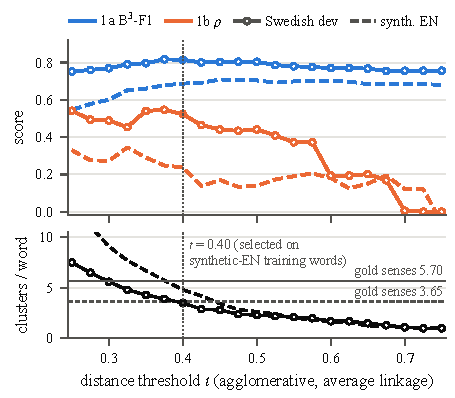
\includegraphics[width=\columnwidth]{figures/threshold}
\caption{Existing method as a function of the distance threshold $t$. Within $t\in[0.30,0.50]$, Swedish \bcubed stays between 0.77 and 0.82, whereas $\rho$ varies by 0.11 on Swedish and by 0.21 on synthetic English.}
\label{fig:threshold}
\end{figure}

\paragraph{How reliable is 1b?}
Figure~\ref{fig:threshold} explains this fragility: within $t\in[0.30,0.50]$, $\rho$ ranges from 0.43 to 0.55 on Swedish and from 0.13 to 0.34 on synthetic English, while Swedish \bcubed stays within 0.77--0.82. With only 60 scored period pairs on Swedish (170 on synthetic English), differences in $\rho$ of a few hundredths are noise. Part of \sys's in-domain gain also comes from calibration alone: a logistic regression on the cosine, fit on synthetic English, with agglomerative clustering reaches $\rho$ 0.284 on synthetic English and 0.540 on Swedish (Appendix~\ref{app:more}). Where the change signal sits matters as well. Only four of the 60 Swedish pairs cross the 1915$\rightarrow$2006 gap, but they are among the largest gold changes (gold ranks 1, 5, 8 and 20; mean distance 0.40 vs.\ 0.21 within an era), and a trivial clustering by era scores $\rho=0.340$ from them alone. Without them, $\rho$ rises to 0.585 for the existing method and 0.552 for \sys: both track within-era dynamics better than the era jump.

\paragraph{Error analysis.}
\sys over-merges: it predicts 2.2--2.9 clusters per Swedish word in Table~\ref{tab:s1}, against 3.5 for the existing method and 5.7 gold senses. This costs most on \emph{suga} `suck', which has 12 gold senses (\bcubed 0.612$\rightarrow$0.434), and \emph{motiv} (0.963$\rightarrow$0.880), but helps \emph{fröken} `miss' (0.809$\rightarrow$0.834; Appendix~\ref{app:words}). The synthetic training words are cleaner: 4.0 senses, modern spelling, no multi-sense usages. Swedish adds an era gap: same-sense pairs from different eras are less similar in \xll space (mean cosine 0.811) than same-sense pairs from one era (0.874), and for \emph{herre} `gentleman, lord' the cross-era value (0.654) approaches that of different-sense pairs (0.532). Historical usages carry OCR errors and pre-1906 spelling (\emph{sorn} for \emph{som}, \emph{lif} for \emph{liv} in an 1883 usage of \emph{kvinna} `woman'), so the encoder separates eras as well as senses. Some senses are not separable at all: for \emph{kvinna}, same- and different-sense pairs are almost equally similar (0.932 vs.\ 0.914), and both systems return one cluster. Figure~\ref{fig:traj} (appendix) shows that \sys reproduces the decline of the minor senses of \emph{herre} after 1915 but merges the title sense of \emph{fru} (\emph{fru Jakobson}), frequent before 1915, with the sense `wife', so its \emph{fru} distribution barely changes.

\begin{table}[t]
\centering
\small
\begin{tabular}{@{}lcc@{}}
\toprule
System & macro-F1 & AUC \\
\midrule
All usages negative & .361 & -- \\
Random (50/50) & .446 & -- \\
\midrule
$\cos(\mathbf{x}_i,\mathbf{g})$ (\emph{existing}) & .571 & .688 \\
Multilingual-E5 sentence cosine & .531 & .640 \\
APPNP propagation of $\cos(\mathbf{x}_i,\mathbf{g})$ & .575 & .695 \\
\sys{} support probability & .579 & .698 \\
One-shot prototype refinement (\emph{ours}) & \textbf{.588} & .704 \\
Few-shot logistic-regression calibrator & .516 & \textbf{.746} \\
\bottomrule
\end{tabular}

\caption{Subtask~2 on Swedish (official per-word macro-F1; AUC averaged over words). Thresholds are chosen on the other nine words; the calibrator is trained on them and labels $p>0.5$ as positive.}
\label{tab:s2}
\end{table}

\paragraph{Subtask 2.}
Prototype refinement improves macro-F1 from 0.571 to 0.588 and AUC from 0.688 to 0.704 (Table~\ref{tab:s2}). It helps most when the usages of the target sense form a coherent group (\emph{motiv} 0.603$\rightarrow$0.891) and hurts when the nearest usages belong to another sense (\emph{förort} `suburb' 0.455$\rightarrow$0.298). The calibrator ranks usages best (AUC 0.746) but has the lowest macro-F1 of the non-trivial systems (0.516): ranking the usages of one word is easier than finding one threshold for all words. The sentence encoder is worse overall (0.531) but the only method that handles \emph{kvinna} (F1 0.647 vs.\ 0.212), whose target sense `women in general' (often \emph{kvinnan}) is less similar to its own definition than the other senses are (\xll AUC 0.33).

% =====================================================================================
\section{Conclusion}

\sys learns the usage graph of a word with few-shot Siamese training and graph message passing; a one-shot prototype detects the usages of a given sense. Message passing clearly improves the learned similarity and gives the best sense dynamics on held-out synthetic English, but on historical Swedish a well-transferred threshold on the frozen \xll cosine remains hard to beat, and the 1b score depends strongly on the threshold and on a few cross-era pairs. Next, we will fine-tune the encoder and train on real annotated usage graphs in several languages.

\section*{Limitations}
The development set has ten words and 60 scored period pairs, so our conclusions about Swedish rest on little data and small differences in $\rho$ are not reliable. Our training data are synthetic English, which differs from the test data in language, noise and sense granularity, and we could not evaluate the five other test languages before the evaluation phase. The encoder is frozen and the output is single-label, both choices dictated by our CPU budget. The development scores of the submitted \sys model are in-sample, since it was adapted on all Swedish development words; every comparison in this paper therefore uses the zero-shot or leave-one-word-out protocols.

\section*{Ethical Considerations}
The data are historical newspapers and modern news text. Several target words (\emph{kvinna}, \emph{fru}, \emph{fröken}, \emph{herre}) denote gendered social roles, and their historical senses reflect the norms of their time. Sense distributions induced by systems like ours can surface such patterns and should be read with this historical context in mind. We see no direct potential for misuse. All experiments ran on a single laptop CPU.

\section*{Acknowledgments}
\acknowledgmentnote We thank the task organisers for the data and the evaluation scripts, and the authors of the synthetic English dataset for releasing it.

\bibliography{references}

% =====================================================================================
\appendix

\section{Hyperparameters}
\label{app:hparams}

\begin{table}[h]
\centering
\small
\begin{tabular}{@{}l>{\raggedright\arraybackslash}p{4.6cm}@{}}
\toprule
Component & Setting \\
\midrule
Encoder & \xll, 128 tokens, mean pooling, frozen \\
Usage graph & $k=10$, edge weights $\max(0,\cos)$ \\
\sys & $d=256$, 2 GNN layers, dropout 0.1 \\
Pair head init. & $s=5$, $a=5$, $b=-6$ \\
Episodes & 1 word $\times$ 128 usages, 2,000 steps \\
Optimiser & AdamW \citep{loshchilov2019decoupled}, lr $3{\cdot}10^{-4}$, weight decay 0.01, one-cycle schedule, gradient clip 1.0 \\
Adaptation & 300 steps, lr $10^{-4}$, 50\% Swedish episodes \\
Corr.\ clustering & 10 restarts, $\le$50 sweeps \\
$\theta$ & seeds: 0.5, 0.6, 0.6; submission: 0.5 \\
Existing method & average linkage, $t=0.40$ \\
Prototype refin. & top 5\% (min.\ 3), 3 rounds, $\tau=0.8625$ \\
APPNP variant & $k=5$, $\alpha=0.5$, 10 steps \\
\bottomrule
\end{tabular}
\caption{Hyperparameters of the submitted systems.}
\label{tab:hparams}
\end{table}

Our correlation-clustering solver starts from pivot clustering, then sweeps over the usages in random order and moves each one to the cluster, or a new singleton, with the largest gain, using incremental node-to-cluster weight sums; it stops when a sweep moves nothing. On 20 random graphs with eight nodes (4,140 partitions each) it reaches the brute-force optimum every time (\texttt{test\_cc\_solver.py}).

\section{Additional Subtask 1 Results}
\label{app:more}

Table~\ref{tab:more} complements Table~\ref{tab:s1}. ``Calibrated cosine'' is a logistic regression from cosine to same-sense probability, fit on the 48 synthetic training words. The choice of $\theta$ on 12 held-out words is itself noisy: the same \sys ensemble obtains $\theta=0.5$ when the grid ends at 0.6 and $\theta=0.7$ when it ends at 0.7. Parameter-free feature smoothing over the $k$NN graph before agglomerative clustering, two steps of $\mathbf{X}\leftarrow\frac{1}{2}\mathbf{X}^{(0)}+\frac{1}{2}\tilde{A}\mathbf{X}$ with the symmetrically normalised adjacency $\tilde{A}$ \citep{wu2019simplifying,gasteiger2019predict}, gives with $k=5$ the highest Swedish $\rho$ of all systems (0.564 zero-shot, 0.548 LOWO) at a small cost in \bcubed.

\begin{table*}[t]
\centering
\small
\begin{tabular}{@{}lcccccc@{}}
\toprule
 & \multicolumn{3}{c}{Synthetic English} & \multicolumn{3}{c}{Swedish dev} \\
\cmidrule(lr){2-4}\cmidrule(l){5-7}
Configuration & B$^3$-F1 & $\rho$ & $k$ & B$^3$-F1 & $\rho$ & $k$ \\
\midrule
\multicolumn{7}{@{}l}{\emph{Similarity $\times$ algorithm ($\theta$ from 12 held-out training words)}} \\
Calibrated cosine + CC ($\theta{=}0.4$) & .674 & .183 & 7.3 & .797 & .549 & 4.9 \\
Calibrated cosine + agglomerative ($\theta{=}0.4$) & .674 & .284 & 6.1 & .810 & .540 & 3.9 \\
\sys{} (ensemble) + CC ($\theta{=}0.7$) & .660 & .201 & 6.0 & .773 & .524 & 3.5 \\
\sys{} (ensemble) + agglomerative ($\theta{=}0.5$) & .694 & .292 & 2.5 & .794 & .414 & 2.2 \\
Mean of both + CC ($\theta{=}0.5$) & .666 & .200 & 5.2 & .789 & .472 & 3.6 \\
Mean of both + agglomerative ($\theta{=}0.5$) & .666 & .252 & 4.5 & .790 & .475 & 3.2 \\
\midrule
\multicolumn{7}{@{}l}{\emph{Seed ensembles + CC}} \\
Siamese head, 3 seeds ($\theta{=}0.5$) & .670 & .161 & 8.0 & .770 & .396 & 4.6 \\
\sys{}, 3 seeds ($\theta{=}0.5$) & .682 & .249 & 3.0 & .785 & .484 & 2.4 \\
\midrule
\multicolumn{7}{@{}l}{\emph{CC at fixed $\theta{=}0.5$ (mean of 3 seeds)}} \\
Siamese head & .670\std{.000} & .181\std{.019} & 7.9 & .769\std{.002} & .435\std{.030} & 4.7 \\
\sys{} & .689\std{.004} & .262\std{.033} & 3.2 & .782\std{.006} & .431\std{.058} & 2.5 \\
\midrule
\multicolumn{7}{@{}l}{\emph{Feature smoothing over the $k$NN graph + agglomerative}} \\
Smoothing, $k{=}5$, 2 steps, $t{=}0.3$ & .684 & .211 & 3.6 & .786 & .564 & 3.2 \\
Smoothing, $k{=}5$, 2 steps (LOWO) & -- & -- & -- & .793 & .548 & 2.8 \\
Smoothing, $k{=}10$, 2 steps, $t{=}0.3$ & .692 & .196 & 3.4 & .784 & .490 & 2.9 \\
Smoothing, $k{=}10$, 2 steps (LOWO) & -- & -- & -- & .768 & .367 & 3.0 \\
\bottomrule
\end{tabular}

\caption{Additional Subtask~1 configurations (official scorer, zero-shot protocol unless marked LOWO).}
\label{tab:more}
\end{table*}

\section{Per-word Analysis}
\label{app:words}

Table~\ref{tab:words} lists, for every Swedish development word, the cluster counts and \bcubed of the existing method and of the zero-shot \sys ensemble (correlation clustering at $\theta=0.5$), and the Subtask~2 scores.

\begin{table*}[t]
\centering
\small
\setlength{\tabcolsep}{4.2pt}
\begin{tabular}{@{}llrrrrrrrrrrr@{}}
\toprule
 & & & & \multicolumn{2}{c}{Clusters $k$} & \multicolumn{2}{c}{1a B$^3$-F1} & & \multicolumn{2}{c}{Subtask 2 F1} & \multicolumn{2}{c}{Subtask 2 AUC} \\
\cmidrule(lr){5-6}\cmidrule(lr){7-8}\cmidrule(lr){10-11}\cmidrule(l){12-13}
Word & Era & $n$ & Gold & Exist. & \sys{} & Exist. & \sys{} & Pos. & Exist. & Proto. & Exist. & Proto. \\
\midrule
\emph{kvinna} `woman' & both & 290 & 5 & 1 & 1 & .787 & .787 & 23\% & .212 & .219 & .327 & .269 \\
\emph{skär} `pure; pink' & early & 98 & 6 & 4 & 2 & .599 & .569 & 28\% & .461 & .508 & .464 & .581 \\
\emph{fröken} `miss' & both & 174 & 4 & 3 & 3 & .809 & .834 & 6\% & .650 & .545 & .800 & .826 \\
\emph{dumpa} `dump' & late & 145 & 6 & 5 & 3 & .890 & .870 & 31\% & .455 & .528 & .587 & .586 \\
\emph{exportera} `export' & late & 149 & 3 & 1 & 2 & .946 & .940 & 95\% & .895 & .853 & .991 & .992 \\
\emph{fru} `wife; Mrs' & both & 274 & 5 & 6 & 2 & .884 & .889 & 89\% & .542 & .569 & .423 & .534 \\
\emph{herre} `gentleman' & both & 283 & 8 & 6 & 5 & .857 & .842 & 7\% & .561 & .567 & .810 & .790 \\
\emph{förort} `suburb' & late & 150 & 3 & 1 & 1 & .804 & .804 & 49\% & .455 & .298 & .537 & .518 \\
\emph{suga} `suck' & late & 129 & 12 & 5 & 3 & .612 & .434 & 19\% & .876 & .901 & .973 & .967 \\
\emph{motiv} `motif' & both & 291 & 5 & 3 & 2 & .963 & .880 & 18\% & .603 & .891 & .971 & .977 \\
\bottomrule
\end{tabular}

\caption{Swedish development words. Era: usages from 1880--1915 (early), 2006--2023 (late) or both. Exist.\ = existing method; Proto.\ = prototype refinement; Pos.\ = share of usages that express the Subtask~2 target sense.}
\label{tab:words}
\end{table*}

\begin{figure*}[t]
\centering
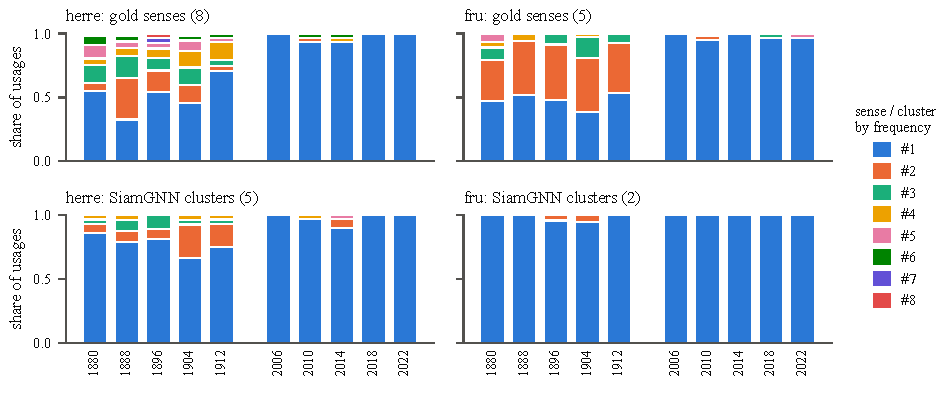
\includegraphics[width=\textwidth]{figures/trajectories}
\caption{Sense distributions per period for \emph{herre} and \emph{fru}: gold senses (top) and clusters of the zero-shot \sys ensemble (bottom), each ranked by overall frequency. The gap separates 1912--1915 from 2006--2007.}
\label{fig:traj}
\end{figure*}

\section{Reproducibility}
\label{app:repro}

{\raggedright
All results can be regenerated with the scripts in \texttt{scripts/}:\par\smallskip
\small
\begin{tabular}{@{}l>{\raggedright\arraybackslash}p{3.0cm}@{}}
\texttt{exp\_main.py} & Table~\ref{tab:s1}; Table~\ref{tab:more}, block 3 \\
\texttt{exp\_subtask1.py} & Table~\ref{tab:s1} (AP, DMoN) \\
\texttt{exp\_hybrid.py} & Table~\ref{tab:s1} (ensemble); Table~\ref{tab:more}, block 1 \\
\texttt{exp\_ensemble.py} & Table~\ref{tab:more}, block 2 \\
\texttt{exp\_graph\_smoothing.py} & Table~\ref{tab:more}, block 4 \\
\texttt{baselines.py} & oracle, era and trivial baselines \\
\texttt{exp\_s2\_final.py} & Table~\ref{tab:s2} \\
\texttt{report\_stats.py} & Table~\ref{tab:words}, Section~5 \\
\texttt{make\_paper\_figures.py} & Figures~\ref{fig:threshold}, \ref{fig:traj} \\
\texttt{test\_cc\_solver.py} & solver check (App.~\ref{app:hparams}) \\
\texttt{build\_report.py} & this paper \\
\texttt{run\_pipeline.py} & submissions \\
\end{tabular}\par}

\end{document}
